\subsection{Experimento 1. Efecto Hall en función de intensidad de corriente}

Representamos gráficamente las medidas tomadas para voltaje al variar la intensidad de corriente manteniendo el campo magnético constante y de valor $B = 250 \pm 1$mT. El efecto Hall en este caso tendrá la forma $V_H = \alpha I$, con lo que identificamos $\alpha = R_H \frac{B}{d} = \frac{B}{nqd}$ con el coeficiente de una regresión lineal.

\begin{figure}[t]
    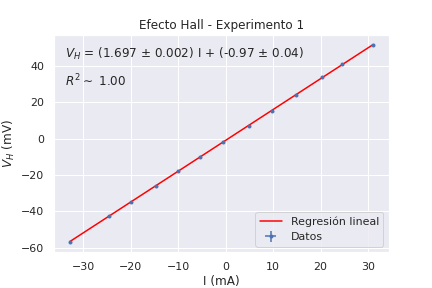
\includegraphics[width=\linewidth]{experimento1}
    \caption{Efecto Hall - Experimento 1: $B = 250 \pm 1$mT}
    \label{figure_exp1}
\end{figure}

La regresión lineal se presenta en la figura (\ref{figure_exp1}), donde obtenemos un buen ajuste al ser $R^2$ my próximo a la unidad, y a partir de la cual calculamos el coeficiente Hall $R_H = (6786.0 \pm 0.3) \cdot 10^{-6}$m/C y la densidad de portadores de carga $n = (9.19 \pm 0.04) \cdot 10^{20}$ portadores/m.

\subsection{Experimento 2. Efecto Hall en función de campo magnético}

Llevamos a cabo el mismo análisis que en el experimento 1, sin embargo, esta vez mantenemos fijado el valor de la intensidad de corriente en $I = 30.0 \pm 0.1$mA y variamos las medidas de campo magnético. En este caso nuestra regresión tendrá la forma $V_H = \beta B$, siendo $\beta = R_H \frac{I}{d} = \frac{I}{nqd}$

\begin{figure}[t]
	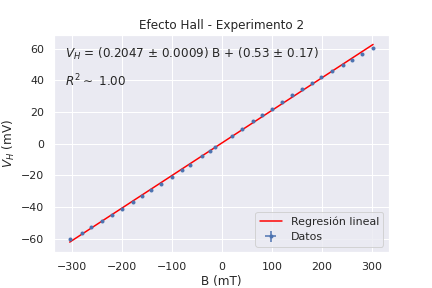
\includegraphics[width=\linewidth]{experimento2}
	\caption{Efecto Hall - Experimento 2: $I = 30.0 \pm 0.1$mA}
	\label{figure_exp2}
\end{figure}

En la figura (\ref{figure_exp2}) presentamos los resultados donde nuevamente el $R^2$ tiende a la unidad. En este caso obtenemos un valor para el coeficiente Hall de $R_H = (6823.1 \pm 0.5) \cdot 10^{-6}$m/C mientras que la densidad de portadores es $n = (9.15 \pm 0.07) \cdot 10^{20}$ portadores/m.

Podemos ver que, aunque los valores obtenidos para la densidad de portadores no comparten cifra significativa, sí ocurre que éstos solapan dentro del error o incertidumbre además de que tienen el mismo orden de magnitud. Concluimos entonces que ambos experimentos ofrecen resultados aceptables.

\subsection{Experimento 3. Efecto Hall y magnetorresistencia}

Manteniendo la intensidad de corriente en $I = 30.0 \pm 0.1$mA medimos voltajes al variar el campo magnético en el rango [0-300mT]. Con estos datos, y partir de la Ley de Ohm, podemos representar gráficamente el cambio relativo de la resistencia frente a su valor inicial $V_0$ cuando $B=0$.

\begin{equation}
	\frac{R - R_0}{R_0} = \frac{V - V_0}{V_0}
\end{equation}

\begin{figure}[t]
	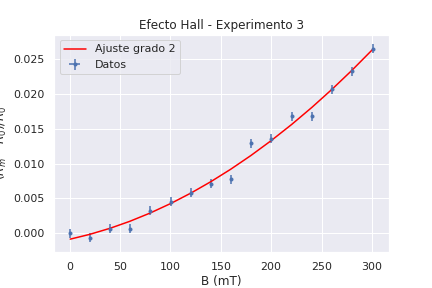
\includegraphics[width=\linewidth]{experimento3}
	\caption{Efecto Hall - Experimento 3: $I = 30.0 \pm 0.1$mA}
	\label{figure_exp3}
\end{figure}

En la figura (\ref{figure_exp3}) se muestran los resultados experimentales sometidos a un ajuste polinómico de segundo orden con coeficientes $1.97 \cdot 10^{-7} B^2 + 3.15 \cdot 10^{-5} B - 8.80\cdot 10^{-4}$. Vemos que la resistencia aumenta de manera no lineal al aumentar el campo magnético, en este caso la relación cuadrática ofrece un ajuste aceptable con un residuo de $r = 1.06 \cdot 10^{-5}$. Este fenómeno se conoce como magnetorresistencia, y es debido a que los conductores en el seno de un campo magnético experimentan una disminución de su conductividad efectiva, al ser desviada parte de la carga que fluye en dirección a la intensidad de corriente.

Gracias a los datos obtenidos podemos estimar la resistencia a temperatura ambiente, cuyo valor es $R_o = 51.6 \pm 0.2 \Omega$. La conductividad viene dada por la expresión

\begin{equation}
	\sigma_o = \frac{l}{R_o \cdot A}
\end{equation}

Con $l$ el largo de la lámina y $A$ la sección transversal. Sustituyendo los valores tenemos $\sigma_o = 38.75 \pm 0.15 \frac{1}{m\Omega}$ y la movilidad $\mu_h = 0.264 \pm 0.003\frac{1}{C\Omega}$

\subsection{Experimento 4. Efecto Hall en función de la temperatura.}

Para comprobar la variación del potencial Hall con la temperatura fijamos la intensidad de corriente en $I = 30.0 \pm 0.1$mA y el campo magnético en $B = 340 \pm 1$mT. Como podemos ver en la figura (\ref{figure_exp4}), el potencial decrece con la temperatura, ya que en este caso el coeficiente Hall depende de la temperatura de manera indirecta a través de la densidad de portadores. Se aprecia en la figura que incluso el potencial llega a invertirse. La explicación a este fenómeno radica en un exceso de huecos frente a portadores electrónicos debido a la transición de semiconductor extrínseco a intrínseco del p-Germanium, rompiendo así condición de la ley de acción de masas.

\begin{figure}[t]
	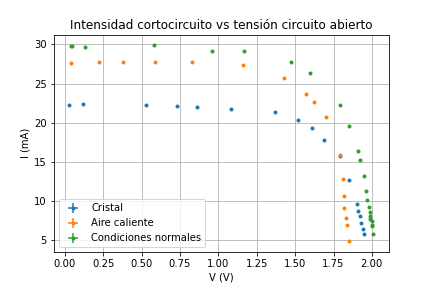
\includegraphics[width=\linewidth]{experimento4}
	\caption{Efecto Hall - Experimento 4: $I = 30.0 \pm 0.1$mA, $B = 340 \pm 1$mT}
	\label{figure_exp4}
\end{figure}

\subsection{Experimento 5. Efecto Hall en función de la temperatura.}

De manera similar al experimento anterior, y con intención de verificar la conductividad del p-Germanium, representamos los datos de $Ln(\frac{1}{V_H})$ frente a $\frac{1}{T}$ en la figura (\ref{figure_exp5}). En ella se presenta el ajuste lineal para la conductividad en la zona intrínseca, dada por $\sigma \propto \frac{1}{V}$, donde la pendiente representa la magnitud $\frac{E_g}{2K_b}$. De esta forma podemos calcular la energía de la banda prohibida de la muestra $E_g = 0.797 \pm 0.003$eV. Siendo el valor teórico para el germanio puro de $E_{g.t} = 0.67$eV tenemos una diferencia de alrededor del 19\%.

\begin{figure}[t]
	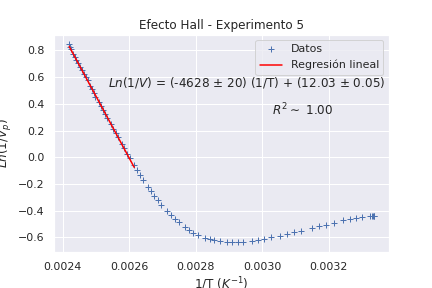
\includegraphics[width=\linewidth]{experimento5}
	\caption{Efecto Hall - Experimento 5}
	\label{figure_exp5}
\end{figure}